\documentclass[12pt]{article}
\usepackage{fullpage,tikz,graphicx}


\usetikzlibrary{automata ,positioning, arrows}


\title{CS 360: Assignment 2}
\author{Cam J. Loader}

\tikzset{
->,% makes the edges directed
node distance=3cm, % specifies the minimum distance between two nodes. Change if necessary.
every state/.style={thick, fill=gray!10}, % sets the properties for each ’state’ node
initial text=$ $, % sets the text that appears on the start arrow
}


\begin{document}
\maketitle

\begin{enumerate}
  \item (10 points) Use the method of eliminating states to find a regular expression for the following
  NFA. The alphabet of the machine is $\sum = {0, 1, 2}$. Draw the initialization step and then draw
  the machine at each step of the process. Eliminate the states in this order: $q1$, $q2$, $q3$, $q4$, $q5$, $q0$.


  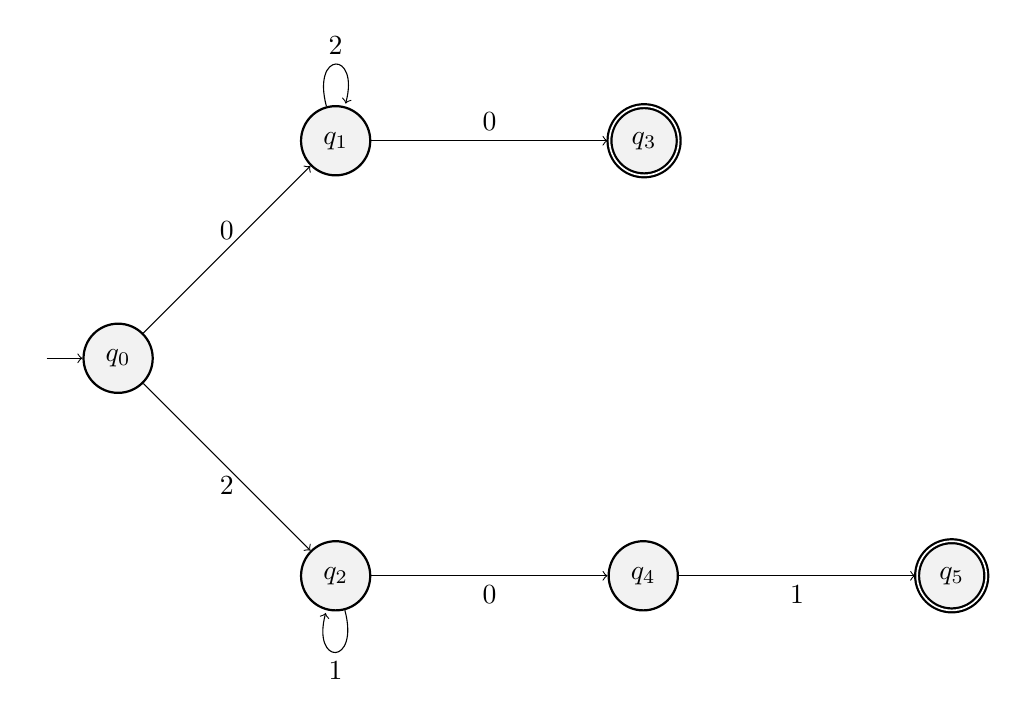
\begin{tikzpicture}
    \node[state, initial] (q0) {$q_0$};
    \node[state, above right=of q0] (q1) {$q_1$};
    \node[state, accepting, right=of q1] (q3) {$q_3$};
    \node[state, below right=of q0] (q2) {$q_2$};
    \node[state, right=of q2] (q4) {$q_4$};
    \node[state, accepting, right=of q4] (q5) {$q_5$};

  \draw (q0) edge[above] node{0} (q1)
        (q1) edge[loop above] node{2} (q1)
        (q0) edge[below] node{2} (q2)
        (q2) edge[below] node{0} (q4)
        (q4) edge[below] node{1} (q5)
        (q2) edge[loop below] node{1} (q2)
        (q1) edge[above] node{0} (q3);

\end{tikzpicture}
  
  Initializing:

  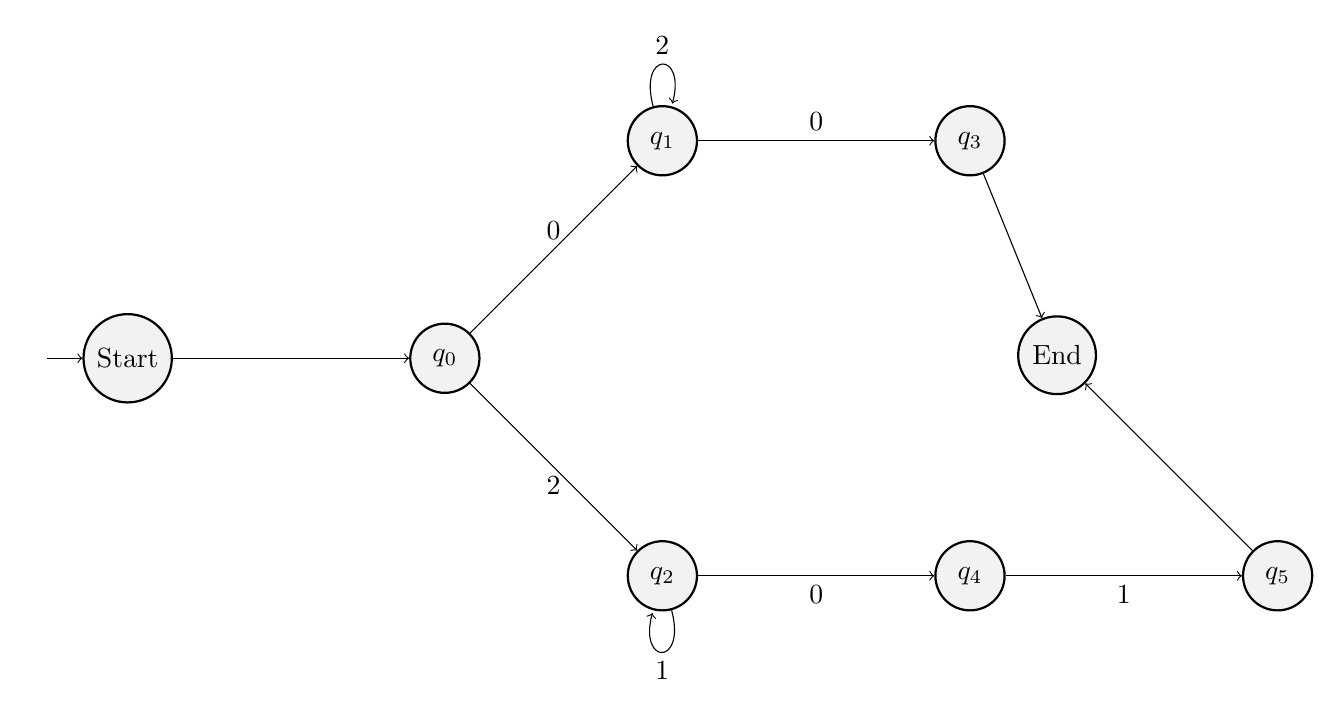
\begin{tikzpicture}
       \node[state, initial] (START) {Start};
       \node[state, right=of START] (q0) {$q_0$};
       \node[state, above right=of q0] (q1) {$q_1$};
       \node[state, right=of q1] (q3) {$q_3$};
       \node[state, below right=of q0] (q2) {$q_2$};
       \node[state, right=of q2] (q4) {$q_4$};
       \node[state, right=of q4] (q5) {$q_5$};
       \node[state, above left=of q5] (END) {End};


     \draw (START) edge[above] node{} (q0)
           (q0) edge[above] node{0} (q1)
           (q1) edge[loop above] node{2} (q1)
           (q0) edge[below] node{2} (q2)
           (q2) edge[below] node{0} (q4)
           (q4) edge[below] node{1} (q5)
           (q2) edge[loop below] node{1} (q2)
           (q1) edge[above] node{0} (q3)
           (q3) edge[above] node{} (END)
           (q5) edge[above] node{} (END);

  \end{tikzpicture}
  $$$$
  
  Removing $q_1$:
  
  \centering 
    \begin{tikzpicture}
            \node[state, initial] (START) {Start};
            \node[state, right=of START] (q0) {$q_0$};
            \node[state, right=of q1] (q3) {$q_3$};
            \node[state, below right=of q0] (q2) {$q_2$};
            \node[state, right=of q2] (q4) {$q_4$};
            \node[state, right=of q4] (q5) {$q_5$};
            \node[state, above left=of q5] (END) {End};

     
         
            \draw (START) edge[above] node{} (q0)
                  (q0) edge[above] node{02*0} (q3)
                  (q0) edge[below] node{2} (q2)
                  (q2) edge[above] node{0} (q4)
                  (q4) edge[below] node{1} (q5)
                  (q2) edge[loop below] node{1} (q2)
                  (q3) edge[above] node{} (END)
                  (q5) edge[above] node{} (END);

  \end{tikzpicture}
$$$$

  Removing $q_2$:
  
  \centering 
    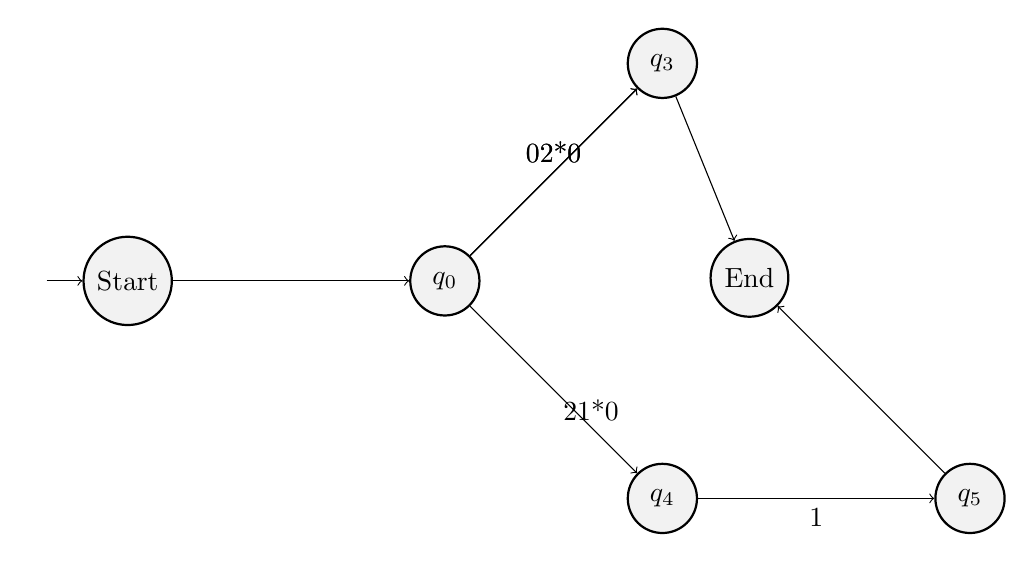
\begin{tikzpicture}
        \node[state, initial] (START) {Start};
        \node[state, right=of START] (q0) {$q_0$};
       \node[state, above right=of q0] (q3) {$q_3$};
       \node[state, below right=of q0] (q4) {$q_4$};
       \node[state, right=of q4] (q5) {$q_5$};
       \node[state, above left=of q5] (END) {End};


       \draw (START) edge[above] node{} (q0)
             (q0) edge[above] node{02*0} (q3)
             (q0) edge[below right=of q0] node{21*0} (q4)
             (q4) edge[below] node{1} (q5)
             (q0) edge[above] node{02*0} (q3)
             (q3) edge[above] node{} (END)
             (q5) edge[above] node{} (END);



  \end{tikzpicture}

$$$$
  Removing $q_3$:
 
    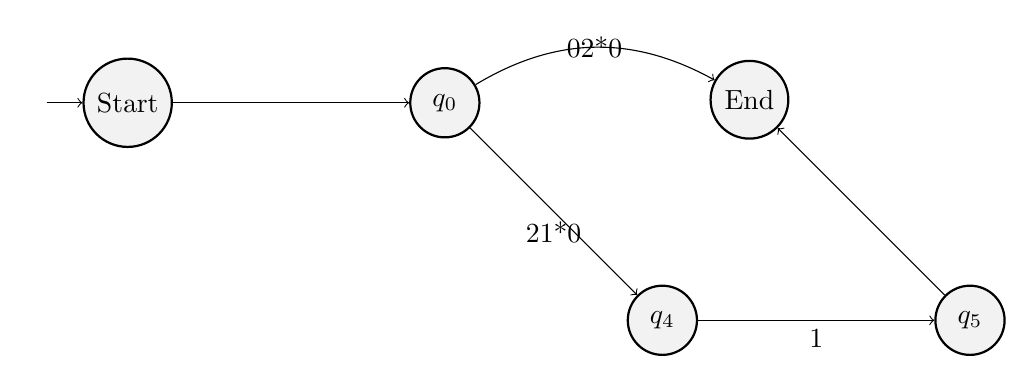
\begin{tikzpicture}
       \node[state, initial] (START) {Start};
       \node[state, right=of START] (q0) {$q_0$};
       \node[state, below right=of q0] (q4) {$q_4$};
       \node[state, right=of q4] (q5) {$q_5$};
       \node[state, above left=of q5] (END) {End};

  
  
       \draw (q0) edge[bend left] node{02*0} (END)
             (START) edge[above] node{} (q0)
             (q0) edge[below] node{21*0} (q4)
             (q4) edge[below] node{1} (q5)
             (q5) edge[above] node{} (END);
    \end{tikzpicture}
  

  Removing $q_4$:
  
  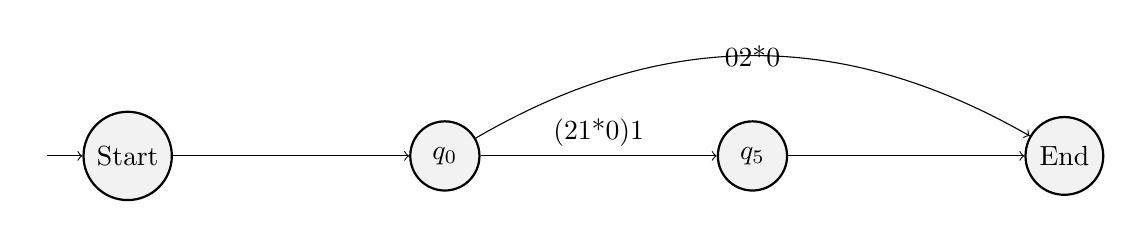
\begin{tikzpicture}
    \node[state, initial] (START) {Start};
    \node[state, right=of START] (q0) {$q_0$};
    \node[state, right=of q0] (q5) {$q_5$};
    \node[state, right=of q5] (END) {End};



    \draw (q0) edge[bend left] node{02*0} (END)
          (START) edge[above] node{} (q0)
          (q0) edge[above] node{(21*0)1} (q5)
          (q5) edge[above] node{} (END);
 \end{tikzpicture}
    Removing $q_5$:
  
    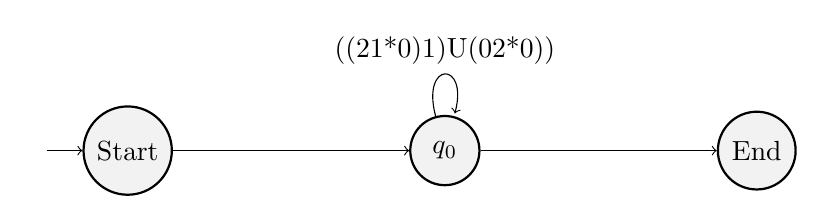
\begin{tikzpicture}
        \node[state, initial] (START) {Start};
        \node[state, right=of START] (q0) {$q_0$};
        \node[state, right=of q0] (END) {End};

    
        \draw (START) edge[above] node{} (q0)
              (q0) edge[loop above] node{((21*0)1)U(02*0))} (q0)
              (q0) edge[above] node{} (END);
     \end{tikzpicture}

    Final regular expression:

    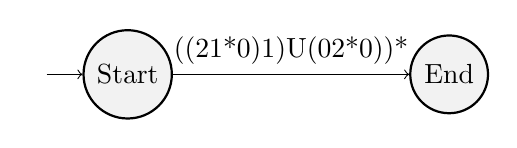
\begin{tikzpicture}
        \node[state, initial] (START) {Start};
        \node[state, right=of START] (END) {End};

    
        \draw (START) edge[above] node{((21*0)1)U(02*0))*} (END);
    \end{tikzpicture}


   \item (10 points) Use the method of eliminating states to find a regular expression for the following
   NFA. The alphabet of the machine is $\sum = {a, b}$. Draw the initialization step and then draw the
   machine at each step of the process. Eliminate the states in this order: $q_0$, $q1$, $q2$, $q3$.
   

   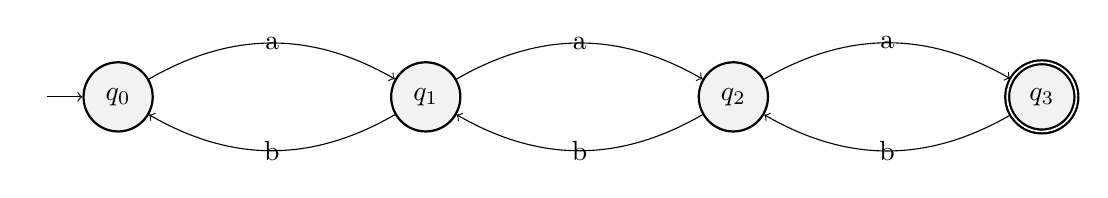
\begin{tikzpicture}
        \node[state, initial] (q0) {$q_0$};
        \node[state, right=of q0] (q1) {$q_1$};
        \node[state, right=of q1] (q2) {$q_2$};
        \node[state, accepting, right=of q2] (q3) {$q_3$};
 
 
      \draw (q0) edge[bend left] node{a} (q1)
            (q1) edge[bend left] node{a} (q2)
            (q2) edge[bend left] node{a} (q3)

            (q3) edge[bend left] node{b} (q2)
            (q2) edge[bend left] node{b} (q1)
            (q1) edge[bend left] node{b} (q0);
   \end{tikzpicture}

Initializing:


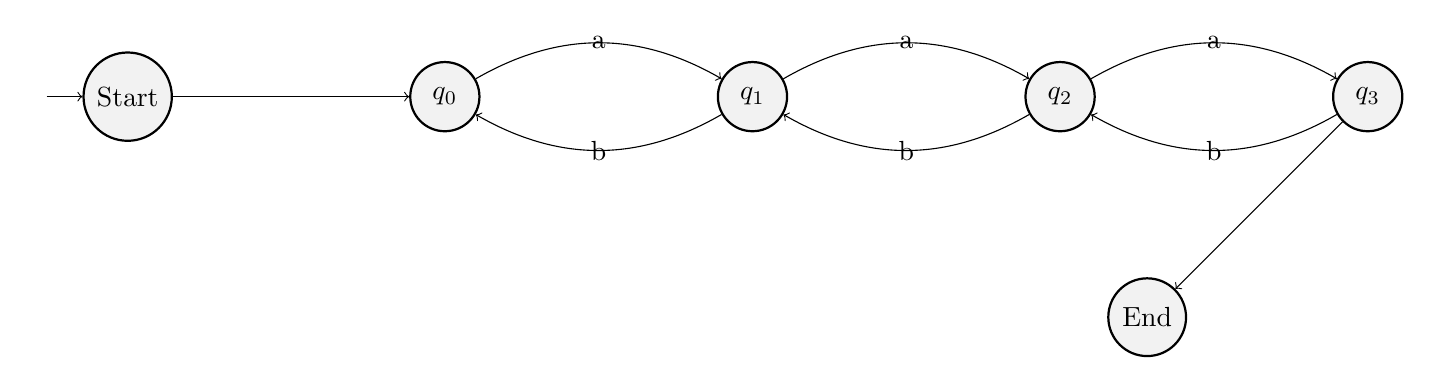
\begin{tikzpicture}
    \node[state, initial] (START) {Start};
    \node[state, right=of START] (q0) {$q_0$};
    \node[state, right=of q0] (q1) {$q_1$};
    \node[state, right=of q1] (q2) {$q_2$};
    \node[state, right=of q2] (q3) {$q_3$};
    \node[state, below left=of q3] (END) {End};


  \draw (START) edge[above] node{} (q0)
        (q0) edge[bend left] node{a} (q1)
        (q1) edge[bend left] node{a} (q2)
        (q2) edge[bend left] node{a} (q3)

        (q3) edge[bend left] node{b} (q2)
        (q2) edge[bend left] node{b} (q1)
        (q1) edge[bend left] node{b} (q0)
        
        (q3) edge[above] node{} (END);
\end{tikzpicture}

Removing $q_0$:

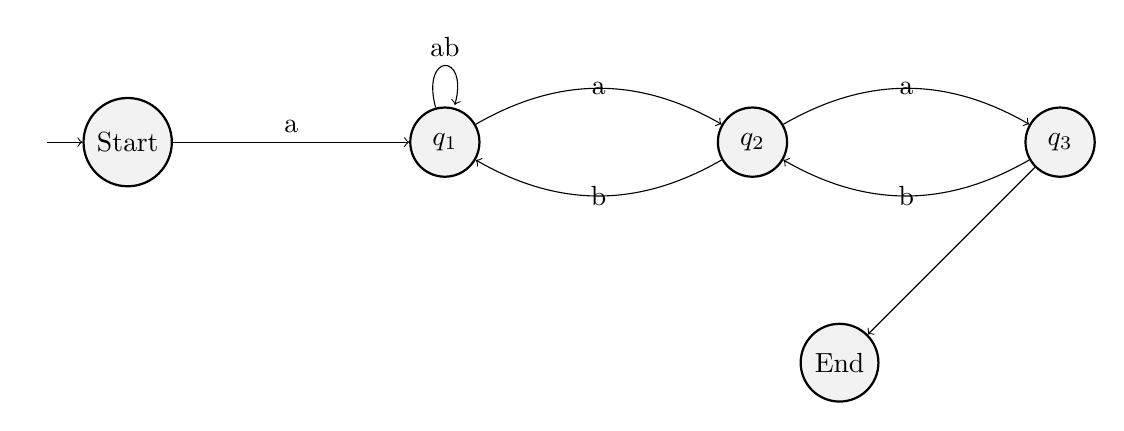
\begin{tikzpicture}
    \node[state, initial] (START) {Start};
    \node[state, right=of START] (q1) {$q_1$};
    \node[state, right=of q1] (q2) {$q_2$};
    \node[state, right=of q2] (q3) {$q_3$};
    \node[state, below left=of q3] (END) {End};


  \draw (START) edge[above] node{a} (q1)
        (q1) edge[bend left] node{a} (q2)
        (q2) edge[bend left] node{a} (q3)
        (q1) edge[loop above] node{ab} (q1)

        (q3) edge[bend left] node{b} (q2)
        (q2) edge[bend left] node{b} (q1)
                
        (q3) edge[above] node{} (END);
\end{tikzpicture}

Removing $q_1$:

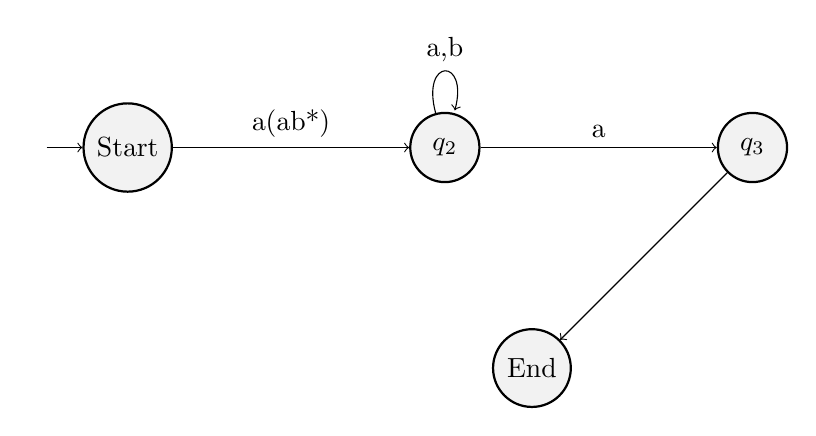
\begin{tikzpicture}
    \node[state, initial] (START) {Start};
    \node[state, right=of START] (q2) {$q_2$};
    \node[state, right=of q2] (q3) {$q_3$};
    \node[state, below left=of q3] (END) {End};


  \draw (START) edge[above] node{a(ab*)} (q2)
         (q2) edge[loop above] node{a,b} (q2)
         (q2) edge[above] node{a} (q3)         
        (q3) edge[above] node{} (END);
\end{tikzpicture}

Removing $q_2$:

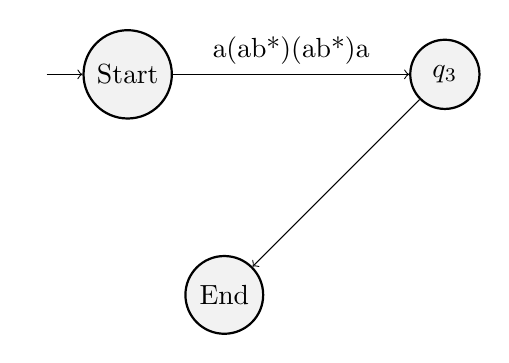
\begin{tikzpicture}
  \node[state, initial] (START) {Start};
  \node[state, right=of START] (q3) {$q_3$};
  \node[state, below left=of q3] (END) {End};


\draw (START) edge[above] node{a(ab*)(ab*)a} (q3)
      (q3) edge[above] node{} (END);
\end{tikzpicture}


Removing $q_3$:

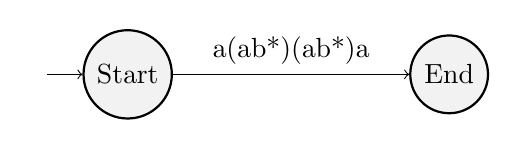
\begin{tikzpicture}
  \node[state, initial] (START) {Start};
  \node[state, right =of START] (END) {End};


\draw (START) edge[above] node{a(ab*)(ab*)a} (END);

\end{tikzpicture}

\end{enumerate}

\end{document}